\documentclass[10pt]{beamer}
\usepackage[UTF8]{ctex}
\usepackage{outlines}
\usepackage{hyperref}
\usepackage{minted}
\usepackage{booktabs}
\usemintedstyle{xcode}
\setminted{
    fontfamily=helvetica
}
\AtBeginSection[]{
  \begin{frame}
  \tableofcontents[currentsection, hideothersubsections]
  \end{frame}
}
\ifx\pdfoutput\undefined
% we are running LaTeX, not pdflatex
\usepackage{graphicx}
\else
% we are running pdflatex, so convert .eps files to .pdf
\usepackage{graphicx}
\usepackage{epstopdf}
\fi

%--------------------------------------------------------
% NOTE: 1) This is an UNOFFICIAL LaTeX beamer style for 
%           Beihang University.
%       2) This is not exactly a beamer style, rather
%           it contains two LaTeX files to be inserted 
%           in the slides' source file.
%       3) These files are based on Edward Hartley's work
%   <http://www-control.eng.cam.ac.uk/Main/EdwardHartley>
%       4) Complaints or suggestions are always welcome.
%
% Xiaoke Yang (das.xiaoke@hotmail.com)
% Wed 15 Jun 11:02:17 CST 2016
%--------------------------------------------------------


%--------------------------------------------------------
% Set up the Beihang University Colours for use with
% xcolor
%--------------------------------------------------------

% Blue palette
\definecolor{coreBlue}{rgb}{0.02 0.30588 0.64706} %#254aa5


%--------------------------------------------------------
% NOTE: 1) This is an UNOFFICIAL LaTeX beamer style for 
%           Beihang University.
%       2) This is not exactly a beamer style, rather
%           it contains two LaTeX files to be inserted 
%           in the slides' source file.
%       3) These files are based on Edward Hartley's work
%   <http://www-control.eng.cam.ac.uk/Main/EdwardHartley>
%       4) Complaints or suggestions are always welcome.
%
% Xiaoke Yang (das.xiaoke@hotmail.com)
% Wed 15 Jun 11:02:17 CST 2016
%--------------------------------------------------------

%--------------------------------------------------------
% Require tikz to do some text positioning
%--------------------------------------------------------
\usepackage{tikz}

%--------------------------------------------------------
% Use Helvetica rather than Computer Modern Sans Serif
% Comment this out if you prefer Computer Modern
%\usepackage{times}
%--------------------------------------------------------
%\usepackage{helvet}

%--------------------------------------------------------
% If you wish to use Arial, and have the winfonts package
% correctly installed uncomment the following to make the
% default sans serif font Arial
%--------------------------------------------------------
%\usepackage{winfonts}
%\usepackage[T1]{fontenc}
%\renewcommand{\sfdefault}{arial}
%--------------------------------------------------------

%--------------------------------------------------------
% Get rid of the navigation bar 
%--------------------------------------------------------
\beamertemplatenavigationsymbolsempty

%--------------------------------------------------------
% Set the files corresponding to the University crests
% here
%--------------------------------------------------------
% Crest with blue text
\newcommand{\beihangcrestblack}{beihangbeamerstyle/beihang-pantone}

% Crest with white text
\newcommand{\beihangcrestwhite}{beihangbeamerstyle/beihang-rev-pantone}
%--------------------------------------------------------

%--------------------------------------------------------
% Define how the page counter will be displayed on slides
%--------------------------------------------------------
\newcommand{\footlinepagecounter}%
	{\insertframenumber{}/\inserttotalframenumber}
%--------------------------------------------------------

%--------------------------------------------------------
% Set up some lengths
%--------------------------------------------------------
% A paper width for the footline
\newlength{\halfpaperwidth}

% The left margin
\newlength{\headingleftmargin}
% Paper width minus margins
\newlength{\headingwidthminusmargins}
% Height of the heading block
\newlength{\headingheight}
% Height of the footer block
\newlength{\footerheight}

% The height for the titlepageheader in the title page
\newlength{\titlepageheaderheight}
% The height for the footer in the title page
\newlength{\titlepagefooterheight}
% The height for the main title block
\newlength{\titlepagemaintitleblockheight}
% The height for the subtitle block
\newlength{\titlepagesubtitleblockheight}
% The height for the name and date block
\newlength{\titlepagenamedateblockheight}
% The height for the institution block
%\newlength{\titlepageinstitutionheight}

% The lengths for spacing between name and date
\newlength{\titlepagespaceundername}
\newlength{\titlepagespaceunderdate}

% The length for the light blue thin bar


\setlength{\headingleftmargin}{0.05573\paperwidth}
\setlength{\headingwidthminusmargins}{\paperwidth}
\addtolength{\headingwidthminusmargins}{-\headingleftmargin}
\setlength{\headingheight}{0.1459\paperheight}
\setlength{\footerheight}{0.09017\paperheight}

\setlength{\titlepageheaderheight}{0.2361\paperheight}
\setlength{\titlepagefooterheight}{0.1459\paperheight}
\setlength{\titlepagemaintitleblockheight}{0.2361\paperheight}
\setlength{\titlepagesubtitleblockheight}{0.1459\paperheight}
\setlength{\titlepagenamedateblockheight}{0.2361\paperheight}
%\setlength{\titlepageinstitutionheight}{0.95cm}

\setlength{\titlepagespaceundername}{16pt}
\setlength{\titlepagespaceunderdate}{8pt}

%--------------------------------------------------------

%--------------------------------------------------------
% Set up the Beihang University blue scheme for use
% with beamer
%--------------------------------------------------------

% Define colour names
\setbeamercolor{coreBlue}{bg=coreBlue, fg=white}

% Set element colours
\setbeamercolor{subtitle}{fg=white}
\setbeamercolor{titlepageheader}{bg=white,fg=black}
\setbeamercolor{titlepagefooter}{bg=white,fg=black}
\setbeamercolor{block title}{bg=white, fg=coreBlue}
\setbeamercolor{structure}{bg=white, fg=coreBlue}
% \setbeamercolor{alerted text}{fg=darkOrange}


%--------------------------------------------------------
% Set font sizes
%--------------------------------------------------------
\setbeamerfont{frametitle}{size=\large,series=\bfseries}
\setbeamerfont{title}{size=\large,series=\bfseries}
\setbeamerfont{author}{size=\normalsize}
\setbeamerfont{date}{size=\scriptsize}
\setbeamerfont{subtitle}{size=\footnotesize,series=\bfseries}
\setbeamerfont{block title}{size=\normalsize,series=\bfseries}
\setbeamerfont{structure}{size=\normalsize,series=\bfseries}

\setbeamertemplate{itemize item}{\scriptsize\raise1.25pt\hbox{\textbullet}}
\setbeamertemplate{itemize subitem}{\scriptsize\raise1.25pt\hbox{\textbullet}}
\setbeamertemplate{itemize subsubitem}{\scriptsize\raise1.25pt\hbox{\textbullet}}


%-----------------------------------------------------
% Define frame title drawing
%-----------------------------------------------------
\setbeamertemplate{frametitle}
{%
  \nointerlineskip
  \begin{beamercolorbox}[wd=\paperwidth,leftskip=\headingleftmargin]{coreBlue}
    \vskip1pt%
    \tikz{\node[minimum height=\headingheight, inner sep=0cm, text width= \headingwidthminusmargins, text badly ragged]{\usebeamerfont{frametitle}\insertframetitle\\\normalsize\it\insertframesubtitle};}
  \end{beamercolorbox}%
}

%-----------------------------------------------------
% Define footline drawing
%-----------------------------------------------------
\setbeamertemplate{footline}
{%
 \setlength{\halfpaperwidth}{0.5\paperwidth}
 \addtolength{\halfpaperwidth}{1pt}
 \leavevmode
 \begin{beamercolorbox}[sep=0pt,wd=\halfpaperwidth, leftskip=\headingleftmargin,right]{coreBlue}
 \tikz{\node[minimum height=\footerheight, inner sep=0cm]{\footlinepagecounter};}%
 \end{beamercolorbox}
 \hskip-1.5pt%
 \begin{beamercolorbox}[sep=0pt,wd=\halfpaperwidth, leftskip=\headingleftmargin, right,rightskip=\headingleftmargin]{coreBlue}
 \tikz{\node[minimum height=\footerheight, inner sep=0cm]{\includegraphics[width=0.25\paperwidth]{\beihangcrestwhite}};}%
 \end{beamercolorbox}%
}


%-----------------------------------------------------
% Define BEIHANG title page
%-----------------------------------------------------
\setbeamertemplate{title page}
{%
\begin{beamercolorbox}[sep=0cm,right,wd=\paperwidth,ht=\titlepageheaderheight,rightskip=\headingleftmargin]{titlepageheader}
\includegraphics[width=0.3820\paperwidth]{\beihangcrestblack}
\vskip0.2361\titlepageheaderheight
\end{beamercolorbox}
\begin{beamercolorbox}[left,leftskip=\headingleftmargin,wd=\paperwidth,ht=\titlepagemaintitleblockheight]{coreBlue}
\tikz{\node[inner sep=0cm, text width=\paperwidth, minimum height=\titlepagemaintitleblockheight,text badly ragged]{\usebeamerfont{title}\inserttitle};}%
\end{beamercolorbox}%
\nointerlineskip%
\vskip-1pt%
\begin{beamercolorbox}[left,leftskip=\headingleftmargin,wd=\paperwidth,ht=\titlepagesubtitleblockheight]{coreBlue}
\tikz{\node[inner sep=0cm, text width=\paperwidth, minimum height=\titlepagesubtitleblockheight, text badly ragged]{\usebeamerfont{subtitle}\usebeamercolor[fg]{subtitle}\insertsubtitle};}%
\end{beamercolorbox}%
\nointerlineskip%
\vskip-1pt%
\begin{beamercolorbox}[left,leftskip=\headingleftmargin,wd=\paperwidth,ht=\titlepagenamedateblockheight]{coreBlue}
      \usebeamerfont{author}\insertauthor\\
      \vskip\titlepagespaceundername%
      \usebeamerfont{date}\insertdate
      \vskip\titlepagespaceunderdate%
    \end{beamercolorbox}%
\begin{beamercolorbox}[left,leftskip=\headingleftmargin,wd=\paperwidth,ht=\titlepagefooterheight]{titlepagefooter}
\end{beamercolorbox}
}


\title{Python入门(一)}
\author{张博涵\\
北京航空航天大学经济管理学院 (\texttt{zhangbohan@buaa.edu.cn})}
\date{\today}

\begin{document}
%----------------------------------------------------------------------
% Title frame
\begin{frame}[plain]
\maketitle
\end{frame}


\begin{frame}
    \frametitle{Outline}
    \tableofcontents
\end{frame}

\section{Python简介}

\begin{frame}
\frametitle{Python简史}

\begin{figure}
    \raisebox{-0.5\height}{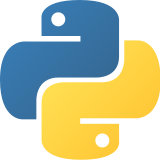
\includegraphics[width=0.3\textwidth]{figures/python.png}}
    \hspace*{2cm}
    \raisebox{-0.5\height}{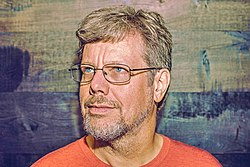
\includegraphics[width=0.3\textwidth]{figures/pythonfather.png}}
\end{figure}

\begin{itemize}
    \item Python是由荷兰程序员``Python之父'' Guido van Rossum 在1989年底开发,并于1991年首次发布Python 0.9.0。
    \item Python 2.0于2000年发布并引入了新功能,在2020年随2.7.18版停止支持。
    \item Python 3.0于2008年发布,并非完全向下兼容,目前的最新正式版本为3.10.5。
\end{itemize}

\end{frame}

\begin{frame}[fragile]
\frametitle{Python特点}
\begin{outline}
    \1 解释型、动态数据类型、自动垃圾回收、可交互
    \1 巨大的、广泛的标准库、强大的社区
        \2 在\href{https://pypi.org/}{pypi}上有388,800个公开项目 
    \1 多范型编程语言,完全支持结构化编程以及面向对象编程,也支持函数式编程和元编程等
    \1 Python的核心采用C语言编写
    \1 代码的可读性强,简单易于上手
\end{outline}

\begin{block}{Python 之禅}
    优美优于丑陋。明了优于隐晦。\quad    简单优于复杂。复杂优于凌乱。 

    扁平优于嵌套。稀疏优于稠密。\quad    可读性很重要。

    \vspace{0.5cm}
    在Python中使用如下代码来输出 The Zen of Python。

    \mint{python}|import this|
\end{block}

\end{frame}

\begin{frame}
    \frametitle{Python 应用}
    \begin{itemize}
        \item Youtube、Reddit、Dropbox、豆瓣、知乎...
        \item 机器学习与人工智能:sklearn, tensorflow, pytorch
        \item 爬虫:requests, scrapy
        \item 云计算:OpenStack
        \item 图形 GUI:PyQT,WXPython,TkInter
        \item 数据分析与科学计算:Numpy, Pandas, Matplotlib
    \end{itemize}
\end{frame}


\section{基本语法}
\begin{frame}[fragile]
\frametitle{基本语法}
Python 3 源码文件以 UTF-8 编码,所有字符串都是 unicode 字符串

\begin{block}{标识符}
    \begin{outline}
        \1 第一个字符必须是字母表中的字母或下划线\mintinline{python}{_}
        \1 标识符的其他的部分由\textbf{字母、数字和下划线}组成。
        \2 这里的字母具体指 UTF-8 字符集中的字符,支持中文(但不建议)
        \2 不能包含 !, \#, @, \$, \%等
        \1 标识符对大小写敏感。
    \end{outline}
\end{block}


\begin{columns}
    \begin{column}{0.5\textwidth}
        \begin{block}{保留字}
            \begin{minted}{python}
            >>> import keyword
            >>> keyword.kwlist
            \end{minted}
            \end{block}
    \end{column}
    \begin{column}{0.5\textwidth}
        \begin{block}{注释}
            单行注释以 \# 开头

            多行注释用 """ 或者 ''' 包裹
        \end{block}
    \end{column}

\end{columns}

\end{frame}


\begin{frame}
\frametitle{基本语法}
\begin{block}{代码块}
\begin{itemize}
    \item Python使用\textbf{缩进}来标识代码块
    \item 一层缩进为一个tab键或者4个空格
    \item 同一个代码块中的代码必须保持相同的缩进,否则报错。
    \item 现代编辑器可以自动缩进
\end{itemize}

\vspace{0.5cm}

\begin{itemize}
    \item Python 代码在执行时从上到下依次执行
    \item 每行代码通常表达一个完整的意思,为一个赋值语句,或者一个表达式,或者调用某个函数
    \item 虽然可以在同一行使用分号分割多个语句,但并不推荐
    \item 若单行代码过长,可以利用反斜杠其分割为多行代码
\end{itemize}
\end{block}
\end{frame}

\begin{frame}
    \frametitle{基本语法}
    \framesubtitle{输入输出 I/O}
    \begin{itemize}
        \item 使用\mintinline{python}{print}输出
        \item 使用\mintinline{python}{input}请求用户的输入
    \end{itemize}

\end{frame}

\section{变量与数据类型}

\begin{frame}
    \frametitle{数据类型}
    \begin{block}{数据类型}
        \begin{itemize}
            \item 数据是存储在计算机中的一串二进制代码
            \item 数据类型代表了这段代码描述了怎样的信息
            \item 例如:数字、字符串、对象、数组、字典等等
        \end{itemize}
    \end{block}
\end{frame}

\begin{frame}
    \frametitle{变量}
    \begin{block}{}
        \begin{itemize}
            \item 变量是指向内存中某块数据的指针,将内存理解为楼房,则变量是每个房屋的钥匙。(堆数据与栈数据)
            \item 变量通过赋值\mintinline{python}{name = value}来进行创建,必须赋值之后才可以被使用或者重新赋值,变量名依照之前的标识符的规则来进行命名。
            \item \mintinline{python}{value} 可以是表达式、字面值、其他变量等等。
            \item Python是动态类型语言,即某个变量可以通过重新赋予新的不同类型的值。赋值以及重新赋值相当于给了变量一把新的钥匙,这个钥匙可能指向同一片数据,也可能指向另一片数据。
        \end{itemize}
    \end{block}

\end{frame}

\begin{frame}
\frametitle{基本数据类型}

\begin{outline}
    \1 数字
        \2 浮点数
        \2 整数
        \2 复数(略过)
    \1 字符与字符串
    \1 布尔型 Boolean
\end{outline}
\end{frame}

\begin{frame}
\frametitle{计算机中数的存储}
\framesubtitle{整数}
\begin{block}{位与字节}
    \begin{itemize}
        \item 位:bit, 一位为一个0或1
        \item 字节: bytes, 1字节 = 8位
    \end{itemize}
\end{block}

\begin{block}{整数存储}
\begin{itemize}
    \item 在计算机中一般用某些固定的长度来存储数字,例如16位,32位,64位,长度越长,存储的范围就越大
    \item 第一位用于表示正负,剩余位数用于表示值,因此16位整数Int16可以表示的范围为 $[-2^{15}, 2^{15}-1]$,例如$0000000000000000$表示$0$, $0111111111111111$表示最大的整数$2^{15}-1$,最特殊的为$1000000000000000$表示最小$-2^{15}$(不需要$+0$以及$-0$)
    \item 一些语言如C语言存在无符号整数UInt,同样位数下表示的范围更大
\end{itemize}
\end{block}

\end{frame}

\begin{frame}
\frametitle{计算机中数的存储}
\framesubtitle{浮点数 float \& double}
\begin{itemize}
    \item 小数采用浮点数的进行存储,整数部分和小数部分分开存储。
    \item 32位浮点数称为单精度浮点数(float),64为浮点数称为双精度浮点数(double)
    \item 浮点数的标准:IEEE-754
\end{itemize}

\begin{table}
    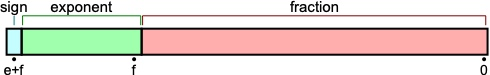
\includegraphics[width=0.8\textwidth]{figures/float.jpg}
\end{table}

\begin{block}{步骤}
    \begin{itemize}
        \item 将数字改写成二进制,$10.75$ => $1010.11$ => $1.01011\times 2^{3}$
        \item 符号位为$0$(1位),指数部分为$3$,实际存储为$3+127=130=10000010_2$(8位),小数部分为$01011000000000000000000$(23位)
        \item 小数部分位数越多,精度越高,但浮点数几乎无法准确表示小数。
    \end{itemize}
\end{block}
\end{frame}

\begin{frame}
\frametitle{Python中的数字类型}
\begin{itemize}
    \item Python中用整数类型为int,浮点数类型为float,存储数的位数自动决定。
    \item 支持其他进制:0x开头为16进制,0b开头为二进制
\end{itemize}

\begin{table}
    \caption{数学计算}
\begin{tabular}{ccc}
    \toprule
    数学计算 & Python符号 & 示例 \\
    \midrule
     $+$ & + & \mintinline{python}{1 + 1.1} \\
     $-$ & - & \mintinline{python}{1 - 1.1} \\
     $\times$ & * & \mintinline{python}{2 * 1.1} \\
     $\div$ & / & \mintinline{python}{2 / 3} \\
     幂 & ** & \mintinline{python}{2 ** 3} \\
     商 & // & \mintinline{python}{5 // 2} \\
     余数 & \% & 5 \% 2 \\
     \bottomrule
\end{tabular}
\end{table}

其他的运算如求对数,通过引入math包进行计算

\mint{python}|import math|

\end{frame}

\begin{frame}
    \frametitle{布尔型}
    \begin{itemize}
        \item bool,表示是(True)或者否(False)
        \item Python中布尔型是整数类型的子类型,可以直接看做数字进行数学运算,True为1,False为0
    \end{itemize}
\end{frame}

\begin{frame}
\frametitle{字符串}

\begin{itemize}
    \item 字符串用于存储一串字符,Python中字符串的类型为\mintinline{python}{str}
    \item 用单引号或双引号直接创建字符串
    \item 可以用\mintinline{python}{[1]}获取特定位置的字符或采用\mintinline{python}{[1:3]}进行范围索引(前闭后开)
    \item 超出索引范围会返回空串而不是报错
    \item Python的整数索引从0开始
    \item 拼接多个字符串:\mintinline{python}{+}
\end{itemize}

\begin{figure}
    \centering
    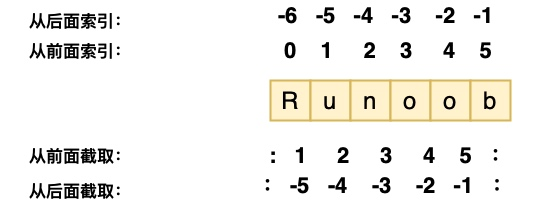
\includegraphics[width=0.5\textwidth]{figures/str_index.jpg}
\end{figure}
\end{frame}

\begin{frame}
    \frametitle{转义字符}

\begin{itemize}
    \item         一些特殊的字符如换行符、tab键等可以通过转义字符来实现,当\mintinline{python}{print}打印字符串或将字符串输出到文件时,转义字符可以发挥作用。
    \item 也可以通过\mintinline{python}{r''}禁止转义
\end{itemize}

    \begin{table}
        \caption{常见的转义字符}
    \begin{tabular}{cc}
    \toprule
    样式 & 含义 \\ \midrule
    \textbackslash n & 换行符 \\
    \textbackslash t & 水平制表符 \\
    \textbackslash ' & 单引号 \\
    \textbackslash r & 回车 \\
    \bottomrule
    \end{tabular}
    \end{table}

    更多详见: \href{https://www.scaler.com/topics/escape-sequence-in-python/}{链接}

\end{frame}

\begin{frame}
    \frametitle{字符串在计算机中的存储}

    编码表:unicode

    编码规则:UTF-8、gbk、gb2312

\end{frame}


\end{document}